\documentclass[11pt]{article}
\usepackage[margin=0.85in]{geometry}
\usepackage{graphicx,booktabs}
\usepackage[hidelinks]{hyperref}
\begin{document}
\section*{Original Model and Defended Model}
The left column shows the Original Model and the right column shows the
Defended Model. The top row shows each model before weight orthogonalization.
The bottom row shows the corresponding orthogonalized snapshot, following
the intervention described by \cite[Sec.~4.1]{arditi2024}.
\section{Non-adversarial prompts}
\begin{table}[ht]
\centering
\caption{Refusal as a harmful-input detector. Harmful input is the positive class. An input is predicted harmful when its refusal metric is strictly greater than zero. Precision is the fraction of positive predictions that are harmful, recall is the fraction of harmful inputs detected, and F1 is their harmonic mean.}
\begin{tabular}{llrrr}
\toprule
Model & Orthogonalization state & Precision & Recall & F1 \\
\midrule
Original Model & Non-orthogonalized & 0.957 & 0.875 & 0.914 \\
Defended Model & Non-orthogonalized & 0.953 & 0.945 & 0.949 \\
Original Model & Orthogonalized & 0.667 & 0.078 & 0.140 \\
Defended Model & Orthogonalized & 0.952 & 0.930 & 0.941 \\
\bottomrule
\end{tabular}
\end{table}
\begin{figure}[p]
\centering
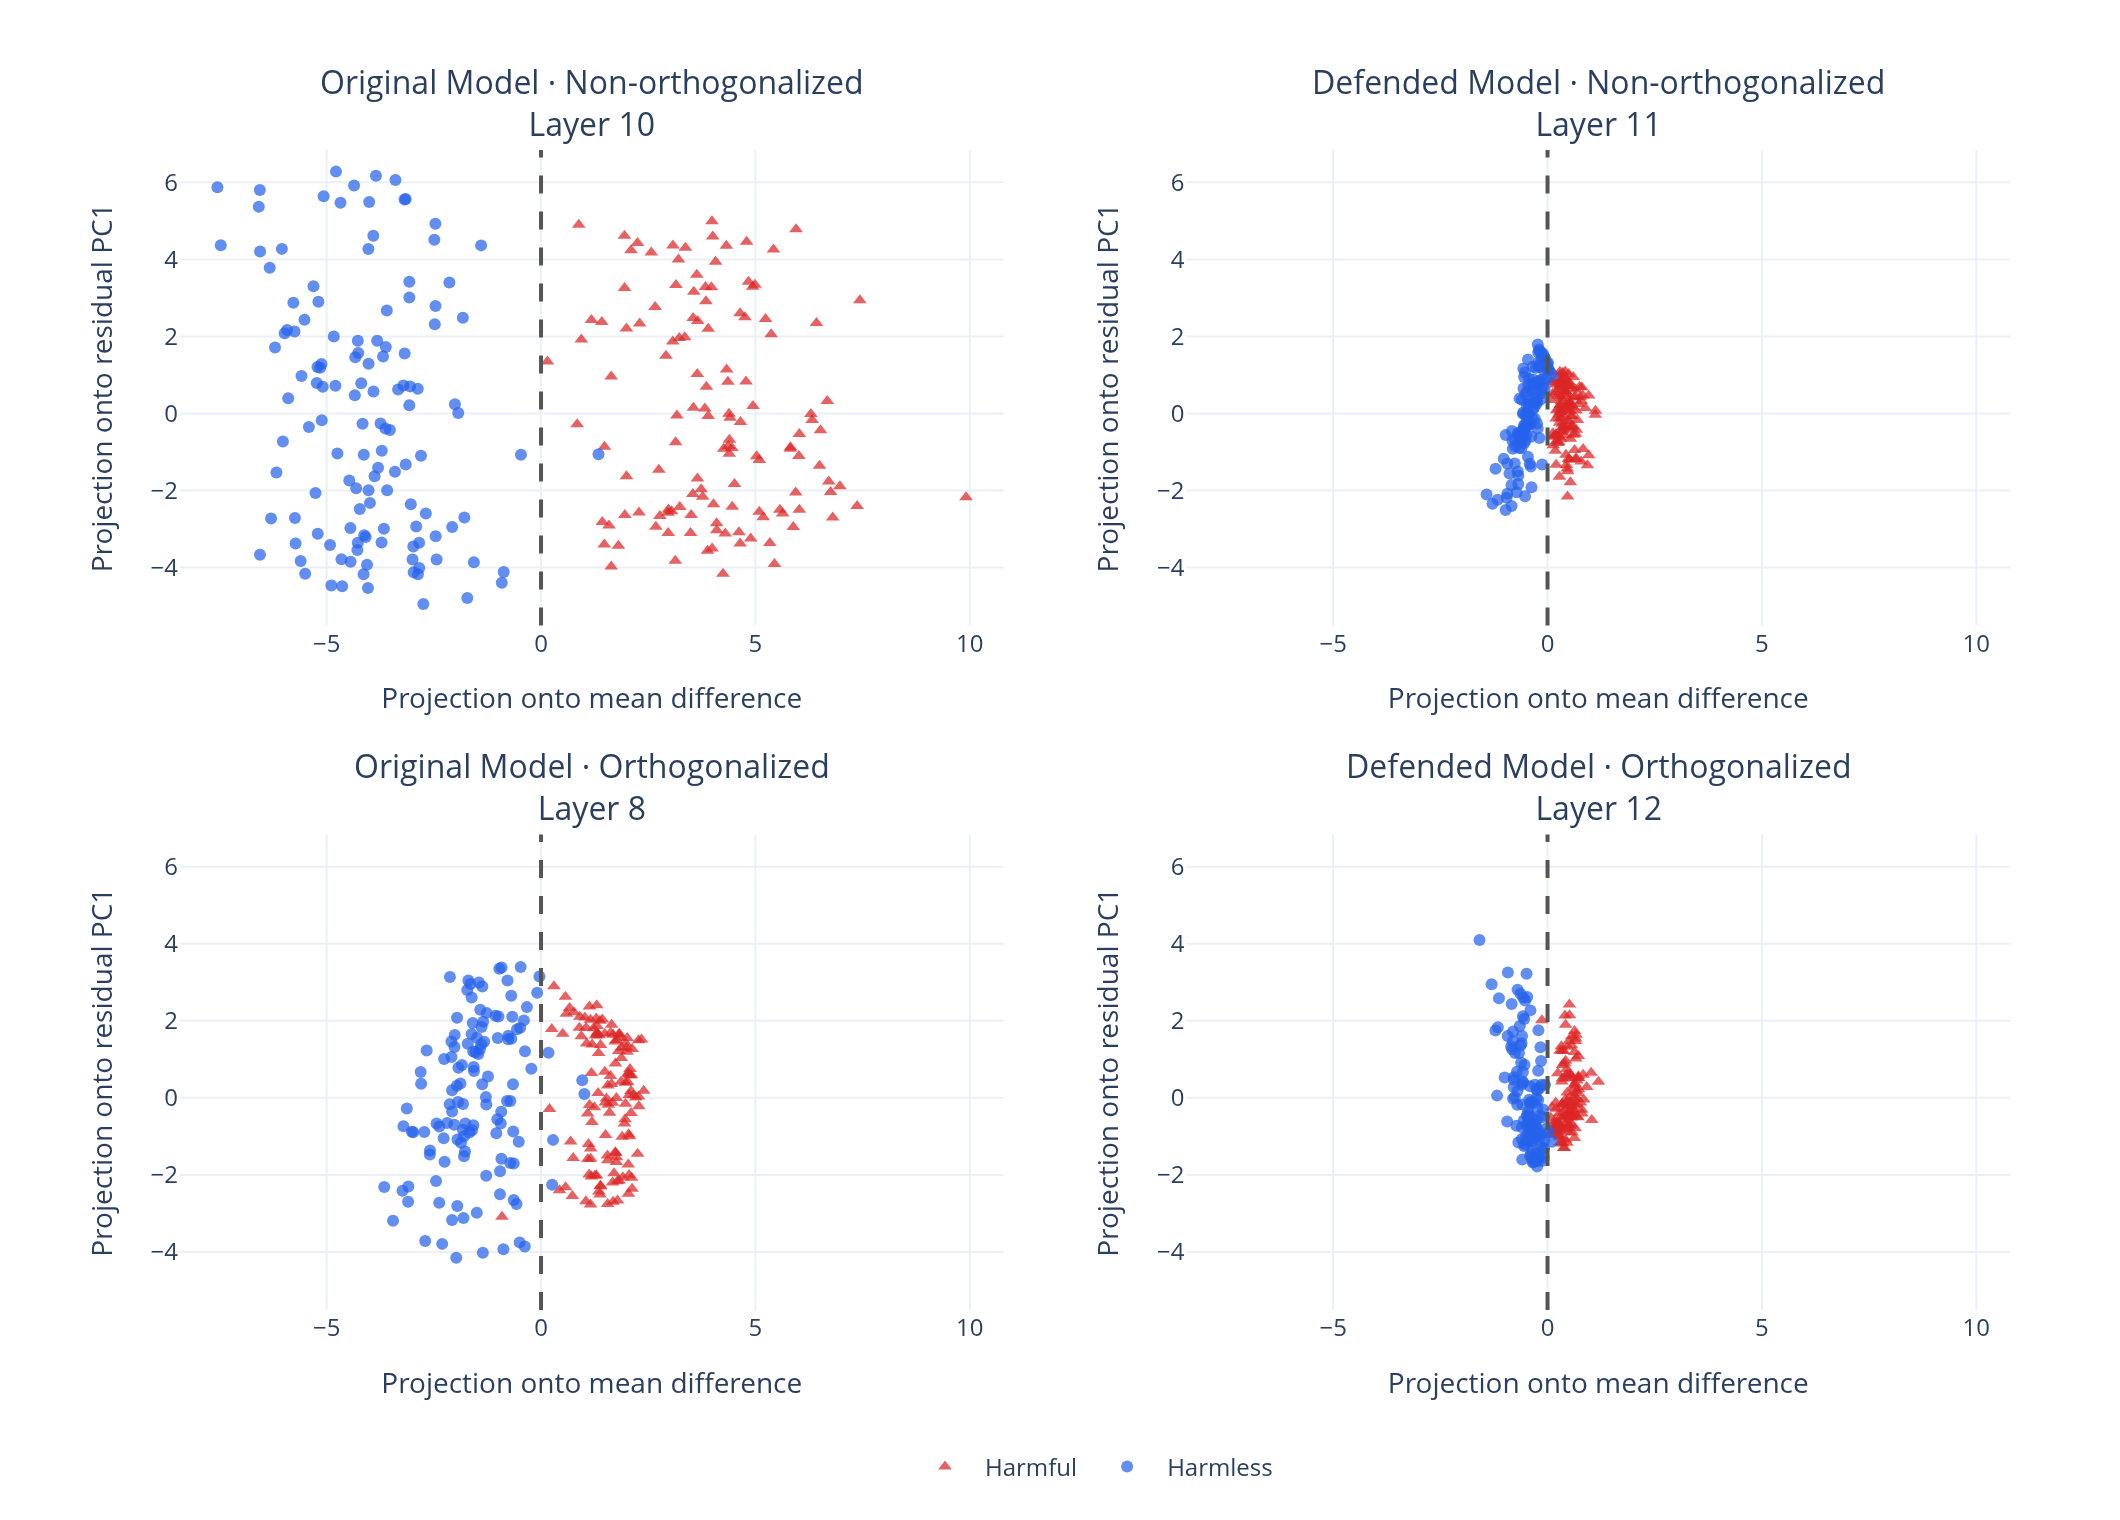
\includegraphics[width=\linewidth]{non_adversarial_scatter_by_class.png}
\caption{\textbf{Activation projections colored by input harmfulness.} Red triangles mark harmful inputs and blue circles mark harmless inputs. Each point is a decoder activation at the final token of the formatted input prompt. The horizontal axis projects the activation onto the unit harmful-minus-harmless mean direction, with zero at the midpoint of the class means. This direction follows the difference-of-means method in \cite[Sec.~2.3]{arditi2024}. The vertical axis projects the centered activation onto the first principal component of the residual after removing its component along that direction. Residual PCA and ranking layers by cross-validated midpoint-classifier F1 are choices of this project. Each panel uses its own best layer (earliest on ties) and its own fitted axes. The common axis limits make the scales comparable across panels.}
\end{figure}
\begin{figure}[p]
\centering
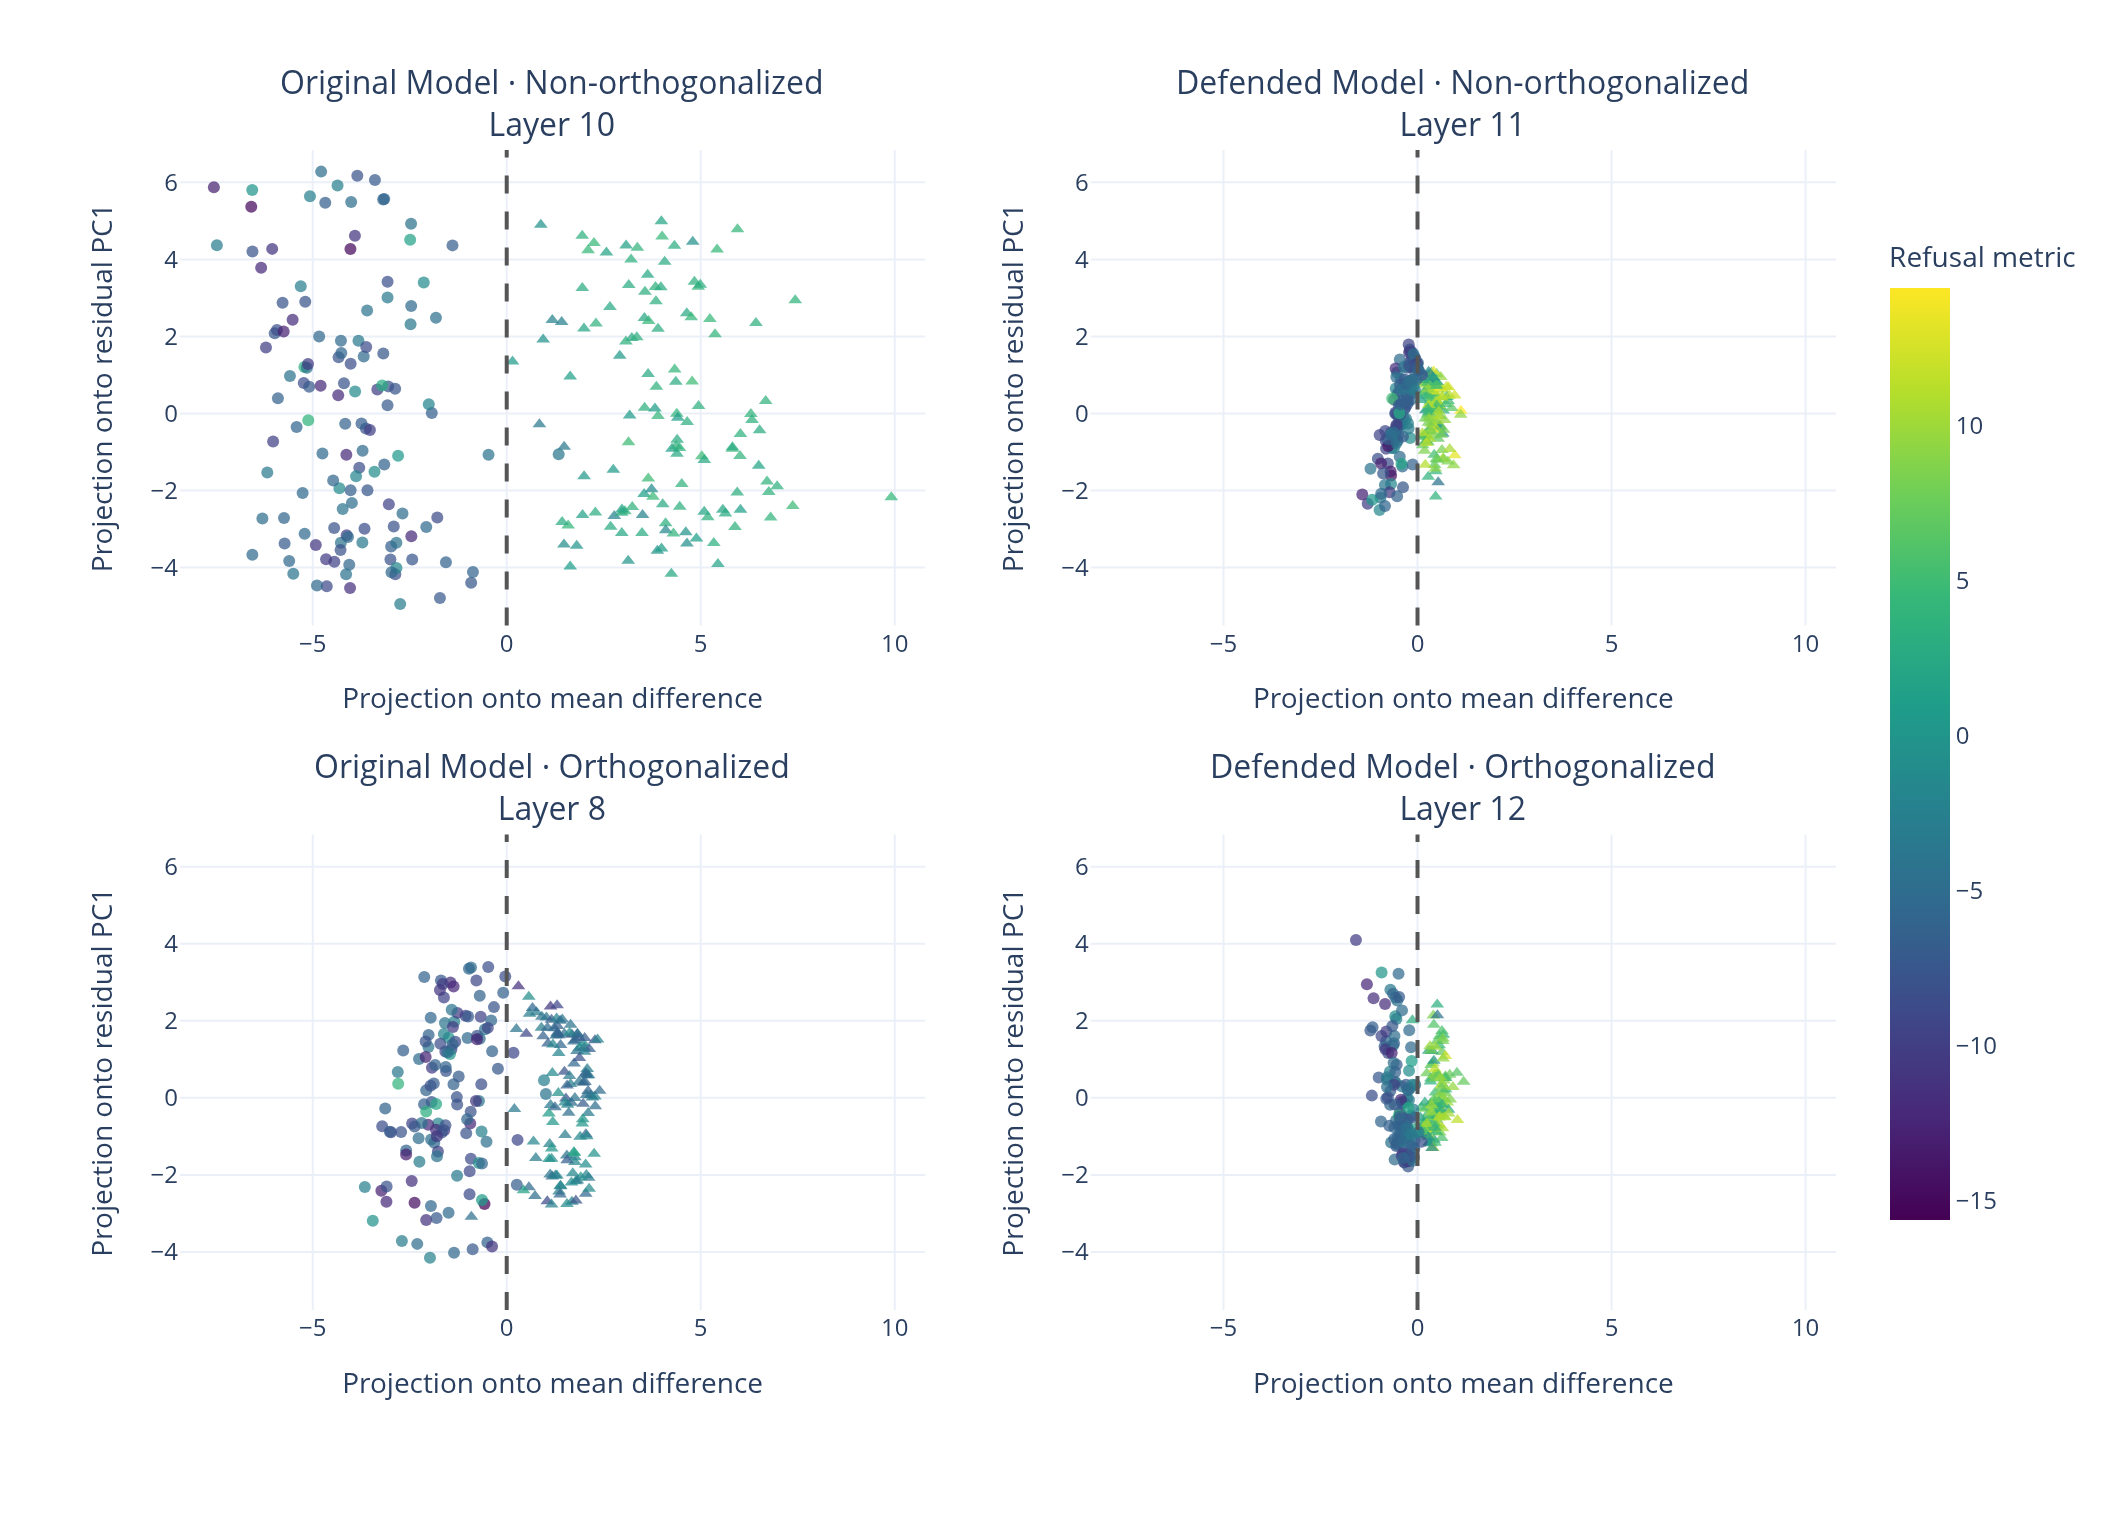
\includegraphics[width=\linewidth]{non_adversarial_scatter_by_refusal_metric.png}
\caption{\textbf{Activation projections colored by refusal metric.} Triangles mark harmful inputs and circles mark harmless inputs. Color indicates the refusal metric on one scale across all panels. The refusal metric is the log odds that the next token belongs to the Qwen Chat refusal set $\{40,2121\}$ \cite[App.~B]{arditi2024}. A positive value means those tokens carry more than half the next-token probability mass. This measures a proxy for refusal from the first response token. Each point is a decoder activation at the final token of the formatted input prompt. The horizontal axis projects the activation onto the unit harmful-minus-harmless mean direction, with zero at the midpoint of the class means. This direction follows the difference-of-means method in \cite[Sec.~2.3]{arditi2024}. The vertical axis projects the centered activation onto the first principal component of the residual after removing its component along that direction. Residual PCA and ranking layers by cross-validated midpoint-classifier F1 are choices of this project. Each panel uses its own best layer (earliest on ties) and its own fitted axes. The common axis limits make the scales comparable across panels.}
\end{figure}
\begin{figure}[p]
\centering
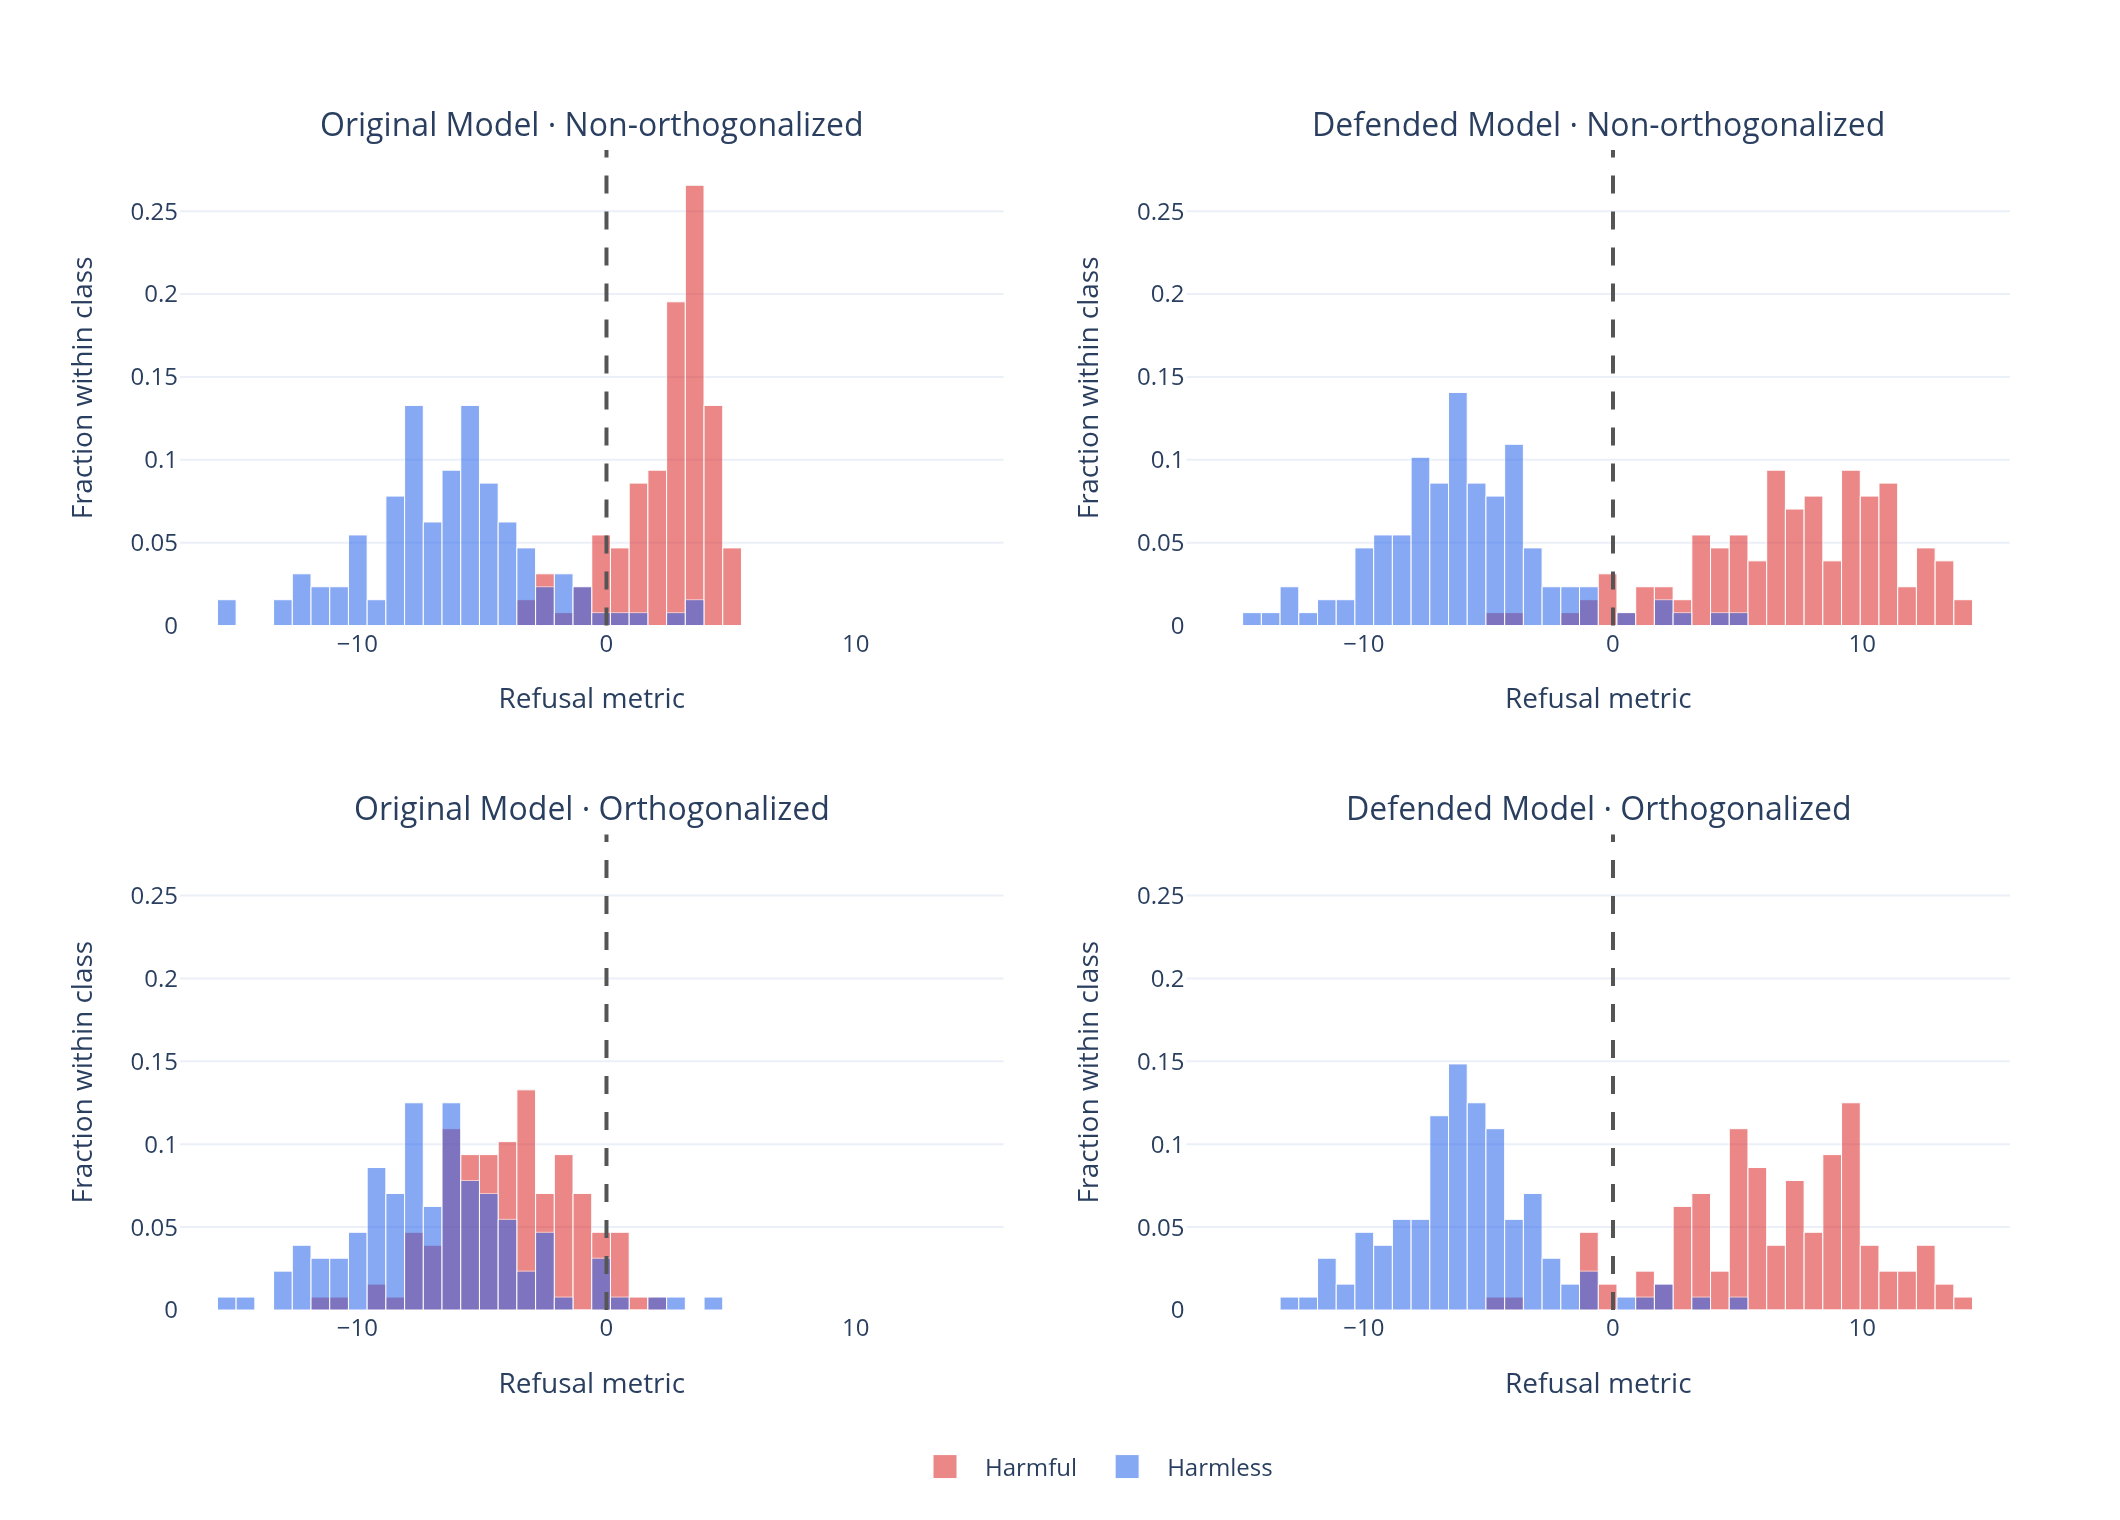
\includegraphics[width=\linewidth]{non_adversarial_refusal_histogram.png}
\caption{\textbf{Empirical refusal metric distributions by input harmfulness.} Red bars show harmful inputs and blue bars show harmless inputs. Bar height is the fraction of examples within that class in each bin. All four panels use the same bin edges and axis limits. The dashed line marks zero, and only values to its right predict harmful input in the detector. The refusal metric is the log odds that the next token belongs to the Qwen Chat refusal set $\{40,2121\}$ \cite[App.~B]{arditi2024}. A positive value means those tokens carry more than half the next-token probability mass. This measures a proxy for refusal from the first response token.}
\end{figure}
\clearpage
\begin{thebibliography}{1}
\bibitem{arditi2024}
A. Arditi et al. (2024).
\href{https://arxiv.org/html/2406.11717v3}{Refusal in Language Models Is Mediated by a Single Direction}.
\end{thebibliography}
\end{document}
